% Title page.
\title[Aula 01]{Oceanografia Física Descritiva}
\subtitle{Histórico da Oceanografia Física}
\author[Filipe Fernandes]{Filipe P. A. Fernandes}
\institute[unimonte]{Centro Universitário Monte Serrat}
\date[Agosto 2013]{09 de Agosto 2013}

\logo{
\includegraphics[scale=0.15]{../common/university_logo.png}}

\begin{document}

% The title page frame.
\begin{frame}[plain]
  \titlepage
\end{frame}

\section*{Outline}
\begin{frame}
\tableofcontents
\end{frame}


\section{Aula 01}
\subsection{Ementa}
\begin{frame}
    \frametitle{Oceanografia Física Descritiva -- Carga horária: 60 h}

    {\bf Ementa} -- Introdução à Oceanografia Física. Conceitos, estrutura e
    características gerais dos oceanos.

    \vspace*{0.5cm}

    {\scriptsize
    {\bf Bibliografia Básica:}
        \begin{itemize}
            \item GARRISON, Tom; MIYAJI, Cíntia (Trad.). Fundamentos de
                oceanografia. São Paulo: Cengage Learning, 2009. 426 p.
                ISBN 9788522106776
            \item MIRANDA, L. B., CASTRO, B. M., KJERFVE, B. 2002. Princípios de
                Oceanografia Física de Estuários. 1a. ed. São Paulo : Edusp, 414p
            \item SVERDRUP, K. A., Duxbury A. B., Duxbury, A. C. 2006. Fundamentals
                of Oceanography. McGraw Hill, 5th edition. Número de Chamada: 551.46 S968f 2006
        \end{itemize}
    }
\end{frame}

\begin{frame}
    \frametitle{Oceanografia Física Descritiva - Carga horária: 60 h}
    {\scriptsize
    {\bf Bibliografia Complementar:}
    \begin{itemize}
        \item STEWART, R. H. 2002. Introduction to Physical Oceanography.
              Department of Oceanography. Texas A. M. University.
              \href{http://oceanworld.tamu.edu/resources/ocng_textbook/contents.html}{link.}
        \item SOUZA, Maria Cristina de Arruda. A Corrente do Brasil ao largo de
              Santos: medições diretas. 2000. 169p. Dissertação  (mestrado).
              Instituto Oceanográfico. USP. Disponível  em:
              http://www.teses.usp.br/teses/disponiveis/21/21132/tde-10092003-094250/pt-br.php
        \item The Open University. 1989. Ocean Circulation, Pergamon Press,
              2nd edition.
        \item TIPLER, Paul Allen. Física para cientistas e engenheiros. 4.
              ed. Rio de Janeiro: LTC, 2006. v.1.
        \item TOMCZAK, Matthias. Physical oceanography. Australia The
              Flinders University of South Australia, 2002. 1 CD-ROM:
              son., color Disponível em:
              http://www.es.flinders.edu.au/~mattom/regoc/pdfversion.html.
    \end{itemize}
    }
\end{frame}

\begin{frame}
    \frametitle{Conversa}
    \begin{itemize}
        \item Lista com nomes e e-mails para contato;
        \item Interesses/Áreas/Estágios;
        \item Nível de Inglês;
        \item Nível de Computação;
        \item Nível de Matemática;
    \end{itemize}
\end{frame}

\begin{frame}
    \frametitle{Avaliações}
    \begin{itemize}[<+-| alert@+>]
        \item 35 + 35 + {\bf 30}.
        \item {\bf 30} divididos entre 15 trabalhos e 15 {\bf TIDIR};
        \item O aluno tem direito a uma prova alternativa (com o conteúdo de
              todo o semestre) para a menor nota.
    \end{itemize}
    \pause
    \begin{block}{}
        Não há segunda chamada{\bf *} nem abono{\bf **}
        de falta não amparado por lei!
    \end{block}
    \pause
    %{\scriptsize {\bf *} O professor não tem a intenção de se colocar
    %entre vocês e uma boa oportunidade de crescimento pessoal.
    %Leia-se: estágios, embarques, congresso e etc podem ser
    %negociados caso-a-caso com MUITA antecedência.}
\end{frame}

\begin{frame}
    \frametitle{Avaliações -- Segunda parte.}
    \begin{itemize}[<+-| alert@+>]
        \item 35 + 35: Serão divididos entre duas provas de 25 e dois sets de sets de avaliações valendo 10;
        \item Provas serão realizadas dias 04/10/2013 e 06/12/2013;
        \item O sets de avaliações deverão ser entregues sempre na próxima aula;
        \item O trabalho de 15 pontos deve ser entregue antes da segunda prova;
        \item Temas para escolher:
    \end{itemize}
\end{frame}

\begin{frame}
    \frametitle{Avaliações -- Segunda parte.}
        \begin{block}{}
        Temas para escolher:
        \end{block}
            {\scriptsize
            \begin{enumerate}[<+-| alert@+>]
                \item Corrente Circumpolar Antártica;
                \item Evolução do modelos de circulação de larga escala;
                \item Massas d'água do Atlântico Sul.
                \item Determinação de massas d'águas "Multi-paramétricas".
                \item O que é a Célula de Revolvimento Meridional?
            \end{enumerate}
            }
\end{frame}

\subsection{Introdução}
\begin{frame}
    \frametitle{O que é a Oceanografia Física?}
    \begin{block}{}
        É o estudo do movimento dos fluidos nos oceanos.  O seu objetivo é o de
        entender os processos nas várias escalas espaciais e temporais, simular
        estes processos e se possível fazer previsões desses.
    \end{block}
\end{frame}

\begin{frame}
    \frametitle{Qual a relevância da Oceanografia Física?}
    \begin{itemize}[<+-| alert@+>]
        \item Os oceanos são uma fonte de alimento.  Processos que influenciam
              os oceanos são importantes para este entendimento, uma vez que
              eles podem atuar como fertilizadores dos oceanos.
        \item Os oceanos são utilizados pelo homem.
            \begin{enumerate}[<+-| alert@+>]
                \item[--] Estruturas são construídas nos oceanos (costa e ao largo);
                \item[--] Os oceanos são utilizados como meio de transporte;
                \item[--] Óleo e gás são obtidos nos oceanos;
                \item[--] Os oceanos também propiciam inúmeras atividades recreativas,
                          tais como: natação, pesca, mergulho, surfe, barco (vela e motor).

            \end{enumerate}
    \end{itemize}
\end{frame}

\begin{frame}
    \frametitle{Qual a relevância da Oceanografia Física?}
    \begin{itemize}[<+-| alert@+>]
        \item Os oceanos influenciam as condições atmosféricas e o clima.
            \begin{enumerate}[<+-| alert@+>]
                \item[--] Distribuição de chuvas, secas, inundações, clima regional,
                          tempestades, furacões e tufões são influenciados pelos oceanos;
                \item[--] Interações oceano-atmosfera são extremamente importantes e
                          ocorrem através dos fluxos de calor e água na superfície oceânica.
            \end{enumerate}
    \end{itemize}
\end{frame}

\begin{frame}
    \frametitle{Como estudar Oceanografia Física?}
    \begin{itemize}[<+-| alert@+>]
        \item O {\bf tema de estudo} exerce uma grande influencia nos tópicos a
              serem estudados dentro da Oc. Fis.
            \begin{enumerate}[<+-| alert@+>]
                \item[--]O que deve ser medido;
                \item[--]Como devem ser feitas as medições;
                \item[--]Quais áreas geográficas de interesse.
            \end{enumerate}
        \item Os {\bf processos} podem ser divididos em:
            \begin{enumerate}[<+-| alert@+>]
                \item[--]Locais;
                \item[--]Regionais;
                \item[--]Globais.
            \end{enumerate}
    \end{itemize}
\end{frame}

\begin{frame}
    \frametitle{Processos locais}
    \begin{center}
      \includegraphics[scale=0.45]{../figures/tunnel.png}
    \end{center}
\end{frame}

\begin{frame}
    \frametitle{Processos regionais}
    \begin{center}
     \shadowbox{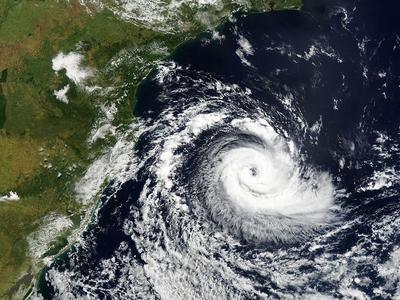
\includegraphics[scale=0.6]{./figures/catarina_1km.jpg}}
%       http://earthobservatory.nasa.gov/NaturalHazards/view.php?id=12935
    \end{center}
\end{frame}

\begin{frame}
    \frametitle{Processos globais}
    \begin{columns}
        \begin{column}{0.5\textwidth}
            \begin{itemize}[<+-| alert@+>]
                \item Os ventos alísios na parte central e oeste do Pacífico
                      enfraquecem;
                \item Termoclina afunda na parte leste e fica mais rasa na
                      parte oeste;
                \item A ressurgência na parte leste fica reduzida, diminuindo
                      aporte de nutrientes;
                \item A TSM aumenta.
    \end{itemize}
        \end{column}
        \begin{column}{0.3\textwidth}
            \centerline{\shadowbox{\includegraphics[scale=0.3]{../figures/elnino.png}}}
            \centerline{\shadowbox{\includegraphics[scale=0.3]{../figures/elnino2.png}}}
        \end{column}
    \end{columns}
\end{frame}

\begin{frame}
    \frametitle{Efeitos globais}
    \begin{columns}
        \begin{column}{0.3\textwidth}
            \centerline{\includegraphics[scale=0.3]{../figures/elnino3_escala.png}}
        \end{column}
        \begin{column}{0.7\textwidth}
            \centerline{\includegraphics[scale=0.45]{../figures/elnino3.png}}
        \end{column}
    \end{columns}
\end{frame}

\subsection{Ferramentas utilizadas no estudo dos oceanos}
\begin{frame}
    \frametitle{Ferramentas utilizadas no estudo dos oceanos}
    \centerline{\includegraphics[scale=0.4]{../figures/ferramentas.png}}
\end{frame}

\subsection{As eras da exploração oceanográficas}
\begin{frame}
\footnotesize{
    \frametitle{A perspectiva histórica}
    \begin{itemize}[<+-| alert@+>]
    \item O conhecimento das correntes oceânicas, dos ventos, das ondas e das
          marés é milenar;
    \item 4000 AC: navegadores da Polinésia já efetuavam relações comerciais a
          longas distâncias no Oceano Pacífico;
    \item 325 AC: Pytheas explorou o Oceano Atlântico indo desde a Itália até a
          Noruega;
    \item Comerciantes árabes usaram o seu conhecimento sobre a reversão dos
          ventos e correntes no Oceano Índico para estabelecer rotas comerciais
          com a China e depois com Zanzibar;
    \item A Conexão das marés com o sol e lua já estava descrita em livros
          indianos entre o período de 2000 a 1400 AC;
    \end{itemize}
}
\end{frame}

\begin{frame}
    \frametitle{A perspectiva histórica}
    \begin{itemize}[<+-| alert@+>]
    \item O conhecimento mais recente dos oceanos, por parte dos europeus, teve
          início com as viagens de:
        \begin{enumerate}[<+-| alert@+>]
            \item Bartolomeu Dias (1487--1488);
            \item Cristóvão Colombo (1492--1494);
            \item Vasco da Gama (1497--1499);
            \item Fernando de Magalhães (1519--1522);
        \end{enumerate}
    \item Tais viagens formaram as fundações para as rotas comerciais globais
          (sec. XVI) e foram baseadas no conhecimento dos seguintes aspectos
          relacionados aos Oceanos Atlântico e Pacífico:
        \begin{enumerate}[<+-| alert@+>]
            \item Ventos Alísios e de Oeste;
            \item Correntes de Contorno Oeste;
                \end{enumerate}
    \end{itemize}
\end{frame}

\begin{frame}
    \frametitle{A perspectiva histórica}
    \centerline{\shadowbox{\includegraphics[scale=0.5]{../figures/ventos.png}}}
\end{frame}

\begin{frame}
    \frametitle{A perspectiva histórica}
    \centerline{\includegraphics[scale=0.4]{../figures/circulacao.png}}
\end{frame}

\begin{frame}
    \frametitle{A perspectiva histórica}
\small{
    \begin{itemize}[<+-| alert@+>]
        \item Os exploradores europeus foram a motivação necessário para o início
            das viagens científicas, tais como:
        \item James Cook (1728--1779) no Endeavour, Resolution e Adventure;
        \item Charles Darwin (1809--1882) no Beagle;
        \item James Clark Ross e John Ross nas regiões Árticas e Antárticas no
            Victory, Isabella e Erebus;
        \item Edward Forbes (1815--1854), que estudou a distribuição vertical dos
            organismos nos oceanos.
        \item Atualmente, as expedições oceanográficas (na medida do possível),
              vem sendo substituídas pelos satélites (?)
    \end{itemize}
}
\end{frame}

\begin{frame}
    \frametitle{As eras da Exploração Oceanográfica}
\small{
    \begin{itemize}[<+-| alert@+>]
        \item Era da Oceanografia Superficial: até 1873. Caracterizada pela
              organização sistemática das observações de vento, correntes,
              ondas, temperatura e outras propriedades obtidas do deck dos
              navios a vela.  Alguns exemplos notáveis são: i) a carta dos
              ventos alísios de Halley, ii) o mapa da Corrente do Golfo de
              Franklin e iii) o livro Physical Geography for the Sea de Matthew
              F. Maury.
        \item Era da exploração do Oceano Profundo: de 1873 a 1914.
        Caracterizada por longas expedições com o intuito de investigar as
        condições superficiais e sub-superficiais dos oceanos. Um exemplo
        deste tipo de expedição foi a Challenger.
    \end{itemize}
}
\end{frame}

\begin{frame}
    \frametitle{As eras da Exploração Oceanográfica}
    \centering{Mapa da rota do H.M.S Challenger (1872--1876)}
    \centerline{\shadowbox{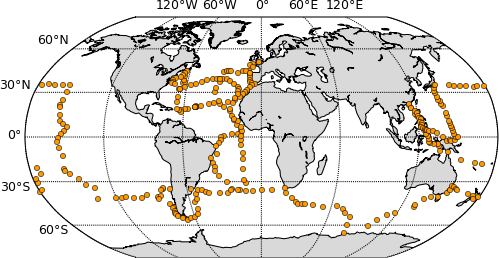
\includegraphics[scale=0.6]{./figures/challenger.png}}}
\end{frame}

\begin{frame}
    \frametitle{As eras da Exploração Oceanográfica}
    \small{Era das campanhas sistemáticas nacionais: de 1925--1940.
    Caracterizada por pesquisas detalhadas em regiões específicas.  Exemplos
    deste tipo de pesquisa são as expedições do {\it Meteor} no Oceano Atlântico
    (1925--1927) e as expedições do {\it Discovery}.}
    \centerline{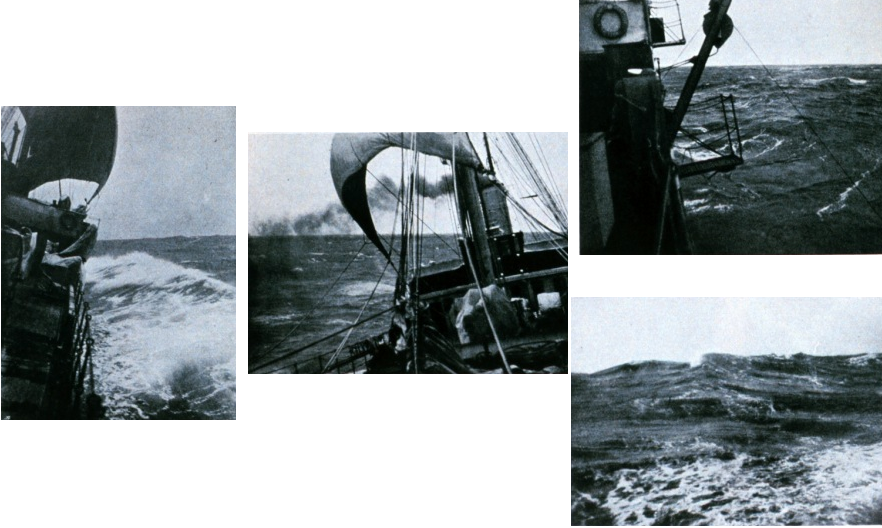
\includegraphics[scale=0.2]{./figures/meteor.png}}
    %     http://www.photolib.noaa.gov/bigs/ship3029.jpg
\end{frame}

\begin{frame}
    \frametitle{As eras da Exploração Oceanográfica}
    \centerline{\includegraphics[scale=0.4]{../figures/meteor_mapa.png}}
\end{frame}

\begin{frame}
    \frametitle{As eras da Exploração Oceanográfica}
    Era dos novos métodos: de 1947--1956.  Caracterizada por longas pesquisas
    com a utilização de novos equipamentos.  Exemplos deste tipo de pesquisa
    incluem as sondagens sísmicas no Oceano Atlântico, no {\it Vema},
    resultando em mapas de relevo submarino.
\end{frame}

\begin{frame}
    \frametitle{As eras da Exploração Oceanográfica}
    \centerline{\shadowbox{\includegraphics[scale=0.45]{../figures/atlantis.png}}}
\end{frame}

\begin{frame}
    \frametitle{As eras da Exploração Oceanográfica}
    Era da Cooperação Internacional: de 1957--1978. Caracterizada por esforços
    de pesquisa envolvendo vários países, com o intuito de estudar os processos
    oceânicos.  Exemplos deste tipo de pesquisa incluem i) o Programa de estudo
    das frentes polares do Oceano Atlântico, ii) os cruzeiros do Ano
    Internacional da Geofísica e iii) a Década Internacional de exploração dos
    oceanos.
\end{frame}

\begin{frame}
    \frametitle{As eras da Exploração Oceanográfica}
    \centerline{\includegraphics[scale=0.25]{../figures/ano_geofisica.png}}
    Examplo da era de cooperação internacional.  Secções no ``International
    Geophysical Year Atlantic Program 1957--1959''.  Adaptado de Wust (1964).
\end{frame}

\begin{frame}
    \frametitle{As eras da Exploração Oceanográfica}
    \begin{itemize}[<+-| alert@+>]
    \item \small{Era dos satélites: de 1978--1995. Caracterizada pelas pesquisas
           globais dos processos oceânicos pelo espaço. Exemplos de alguns
           destes satélites incluem: Seasat, NOAA 6-10, NIMBUS-7, Geosat,
           Topex/Poseidon e ERS 1 e 2.}

    \item \small{Era da Ciência Global: de 1995 - presente. Caracterizada por
           estudos globais com a finalidade de investigar a interação dos
           processos biológicos, químicos e físicos no oceano e atmosfera e na
           parte terrestre. Tais estudos agregam dados in situ e dados de
           satélite para validar modelos numéricos. Exemplos destes programas
           incluem o World Ocean Circulation Experiment (WOCE) e o
           Topex/Poseidon.}
    \end{itemize}
\end{frame}

\begin{frame}
    \frametitle{As eras da Exploração Oceanográfica}
    \centerline{\shadowbox{\includegraphics[scale=0.45]{../figures/woce.png}}}
\end{frame}

\begin{frame}
    \frametitle{As eras da Exploração Oceanográfica}
    \centerline{\shadowbox{\includegraphics[scale=0.45]{../figures/topex.png}}}
\end{frame}

\subsection{Considerações finais}
\begin{frame}
    \frametitle{Considerações finais}
\small{
    \begin{itemize}[<+-| alert@+>]
        \item Os oceanos são pouco conhecidos.  O que se conhece é baseado em
              dados coletados a pouco mais de um século e que a partir de 1978,
              vem sendo complementados com observações de satélite;
        \item Um descrição básica do oceano é suficiente apenas para descrever
              a circulação média dos oceanos.  Recentemente, um grande esforço
              vem sendo colocado para descrever a variabilidade destes processos;
        \item As observações são essenciais para se entender os oceanos.
              Poucos processos foram previstos a partir da teoria, sem ter sido antes observados.
    \end{itemize}
}
\end{frame}

\begin{frame}
    \frametitle{Considerações finais}
    \centerline{\includegraphics[scale=0.4]{../figures/woa_temp.png}}
\end{frame}

\section{Exercícios}
\begin{frame}
    \frametitle{Dimensão dos oceanos}

    \small{Os oceanos e áreas adjacentes cobrem 70.8\% da superfície da Terra.
    As dimensões oceânicas varia de $\approx$1500 km para a largura mínima do
    Atlântico até mais de 13000 km para a extensão norte-sul do Atlântico e
    largura do Pacífico.  Profundidades típicas estão entre 3--4 km.}

    \begin{itemize}[<+-| alert@+>]
        \item Oceano Pacífico: 181,34 $\times$ 10$^6$ km$^2$
        \item Oceano Índico: 74,12 $\times$ 10$^6$ km$^2$
        \item Oceano Atlântico: 106,57 $\times$ 10$^6$ km$^2$
    \end{itemize}
\end{frame}


\begin{frame}
    \frametitle{Dimensão dos oceanos}
    \centerline{\shadowbox{\includegraphics[scale=0.45]{../figures/papel.png}}}
\end{frame}


\begin{frame}
    \frametitle{(1/3) Dimensão dos oceanos}

    \small{As dimensões horizontais das bacias dos oceanos são 1000
    vezes maior que as dimensões verticais.
    Como seria um modelo de escala para o do Pacífico?
    % Esse modelo teria dimensões similares a uma folha de papel:
    % uma largura de 10000 km para 25.4 cm, e a profundidade de 3 km para
    % 0,007 cm, a largura típica de uma folha de papel.
    }
    \pause

    \begin{block}{}
      \bf{Porque isso é importante?  Quais implicações para a circulação?}
    \end{block}
\end{frame}

\begin{frame}
    \frametitle{(2/3) Gota e água doce em uma amostra oceânica}
    \begin{block}{}
        \bf{Se adicionarmos uma gota* de água doce em uma amostra de
        200 mL de água do mar**, qual seria a nova salinidade dessa mistura?}
%         \[
%             \frac{200}{200 + 0,025} \times 35 =  34,996.
%         \]
    \end{block}
    * 1 gota tem aproximadamente 0,025 mL de água.\\
    ** Use 35 g/Kg para a salinidade da água do mar.
\end{frame}


\begin{frame}
    \frametitle{(3/3) Equipamentos oceanográficos}
    \begin{block}{}
        Escolha um equipamentos oceanográfico e:
        \begin{itemize}
          \item Descreva o equipamento, seu uso e  princípio de funcionamento;
          \item Levante o preço do mesmo, suas vantagens e desvantagens e uma
                alternativa (outro equipamento e/ou técnica de medida).
        \end{itemize}
    \end{block}
\end{frame}

\end{document}
